\par En ciertos proyectos, el alcance del software es muy grande para desarrollarse de forma lineal. También puede suceder que es necesario entregar un software funcional en un corto plazo \cite{pressmanIngenieriaSoftwareEnfoque2013}. Para estos casos se pueden utilizar los modelos incrementales.
\par En este tipo de modelos, el software se avanza a partir de entregas incrementales, donde cada incremento suma nuevas funcionalidades. Generalmente, las primeras entregas incluyen los requerimientos urgentes, de forma que el cliente pueda validarlos en una etapa temprana del desarrollo \cite{sommervilleIngenieriaSoftware9a2011,pressmanIngenieriaSoftwareEnfoque2013}.
\par Cada uno de estos incrementos sigue el ciclo de vida en cascada, es decir que el desarrollo de una iteración se separa en módulos que deben ser terminados para avanzar al siguiente \cite{gujarathiSpiralDevelopmentNonSoftware2024}.
%
\begin{figure}[h]
  \centering
  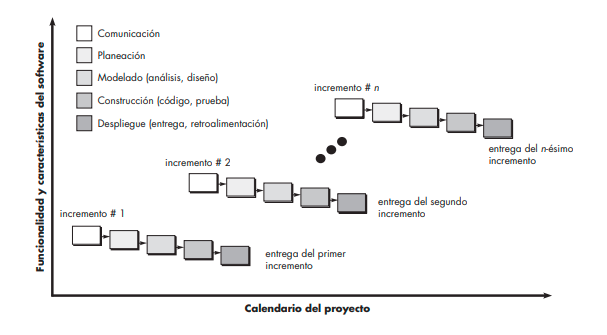
\includegraphics[scale=0.8]{image5.png}
  \caption{Modelo incremental . Extraída de \cite{pressmanIngenieriaSoftwareEnfoque2013}.}
  \label{fig:x Modelo incremental}
\end{figure}
\par El desarrollo incremental es particularmente útil cuando no se dispone del personal para la implementación completa del producto. Un equipo pequeño puede crear una versión básica del proyecto, y escalar a medida que la empresa crece \cite{pressmanIngenieriaSoftwareEnfoque2013}. 
Sin embargo, ciertas desventajas aparecen con este tipo de metodologías. En un principio, es difícil medir el progreso de un proyecto cuando las entregas se crean en rápida sucesión. A esto se suma que la estructura del sistema tiende a degradarse con el paso del tiempo debido a la periodicidad de cambios \cite{sommervilleIngenieriaSoftware9a2011}.
